\setcounter{part}{13}  % E

\part{\'Electromagnétisme}
\section{Induction}
\begin{exercise}{Rail de Laplace}{1}{Sup}
{Induction}{lelay}

On considère un rail de Laplace (dans un champ $\vec{B} = B_0\ve_z$, une barre conductrice placée en $x_0 > 0$ dans la direction $y$ perpendiculairement à une paire de rails dirigés selon $Ox$, écartés d'une distance $a$ et reliés en $x = 0$ par une résistance $R$).

\begin{questions}
    \questioncours Loi de Lenz
    \question On donne à la tige une vitesse initiale $v_0$. 
    \begin{parts}
        \part Sans calcul, quelle sera la vitesse de la barre lorsque $ t \rightarrow \infty$ ?
        \part Donner la durée caractéristique d'évolution de la vitesse de la barre.
    \end{parts}
    \question Pour cette question, on ne donne pas de vitesse initiale mais un opérateur applique une force constante de norme $F_0$ sur la barre.
    \begin{parts}
        \part Quelle sera la vitesse de la barre lorsque $ t \rightarrow \infty$ ?
        \part Quelle est aux temps longs la puissance dissipée dans la résistance ?
    \end{parts}
    \question Pour cette question, on n'applique pas de force mais on remplace la résistance de la barre par une bobine d'inductance $L$. Quelle énergie faut-il pour déplacer la barre sur une distance $D$ ?
\end{questions}

\end{exercise}

\begin{exercise}{Rails de Laplace inclinés}{2}{Sup}
{Induction}{lelay}

On considère un rail de Laplace (dans un champ $\vec{B} = B_0\ve_z$, une barre conductrice est placée en $x_0 > 0$ dans la direction $y$ perpendiculairement à une paire de rails dirigés selon $Ox$, écartés d'une distance $a$ et reliés en $x = 0$ par une résistance $R$).

\begin{questions}
    \questioncours Principe d'induction.
    \question On donne à la tige une vitesse initiale $v_0$. 
    \begin{parts}
        \part Sans calculs, quelle sera la vitesse de la barre lorsque $ t \rightarrow \infty$ ?
        \part Donner le temps caractéristique d'évolution de la vitesse de la barre.
    \end{parts}
    \question Cette fois on ne donne pas de vitesse initiale et on incline les rails d'un angle $\alpha$, de manière à ce que la barre subisse une force $g\sin(\alpha)$ la poussant vers l'avant.
    \begin{parts}
        \part Quelle sera la vitesse de la barre lorsque $ t \rightarrow \infty$ ?
        \part Donner le temps caractéristique d'évolution de la vitesse de la barre.
    \end{parts}
    \question Est-il raisonnable de supposer que les rails n'ont pas de résistance ? On suppose maintenant qu'ils sont chacun dotés d'une résistance linéique $\rho/2$.
    \begin{parts}
        \part Quelle différence par rapport à la question précédente ?
        \part Quelle sera la vitesse de la barre lorsque $ t \rightarrow \infty$ ?
        \part Donner le temps caractéristique d'évolution de la vitesse de la barre.
    \end{parts}
    \question Même question pour des rails divergents (au lieu d'être parallèles, ils sont écartés d'un angle $\alpha$).
\end{questions}

\end{exercise}
\begin{exercise}{Mesure de mutuelle}{2}{Sup}
{Induction,Bobines}{lelay}

On dispose de deux bobines d'inductance propre $L = 10$~mH et d'inductance mutuelle $M$. On cherche à mesure cette inductance propre. Pour ce faire, une des bobines est mise en série avec une résistance $R = 100$~$\Omega$ et un GBF fournissant une tension $e(t)$. On mesure la tension $u(t)$ aux bornes de la seconde bobine à l'aide d'un  voltmètre.

\begin{questions}
    \questioncours Loi de Faraday pour les bobines
    \question Exprimer $u(t)$ en fonction du courant $i(t)$ passant à travers la résistance et de l'inductance mutuelle entre les deux bobines $M$.
    \question Comment doit-on choisir la fréquence d'oscillation $f$ pour que le courant $i(t)$ soit proportionnel à $e(t)$ ?
    \question Le GBF délivre une tension triangulaire oscillant entre $-10$~V et $+10$~V à la fréquence $f = 100$~Hz. La tension mesurée $u(t)$ a une valeur efficace de $40\pm 5$~mV. En déduire une estimation de l'inductance mutuelle $M$.
\end{questions}

\end{exercise}

\begin{solution}
    
\begin{questions}
    \questioncours Loi de Faraday pour les bobines
    \question $u = M\dv{i}{t}$
    \question Dans le circuit avec le GBF on a (loi des mailles) $e = Ri + L\dv{i}{t}$. On veut $i\propto e$ donc $R i \gg L\dv{i}{t}$ i.e. $R\gg L\omega$ soit $f \ll R/(2\pi L)$
    \question En combinant les deux relations on a $u = \frac{M}{R}\dv{e}{t}$. La tension $e$ change de 20~V en une demie période soit 5~ms, d'où $\dv{e}{t} = 4$~kV/s. Le signal $u$ est la dérivée d'un signal triangle, donc un signal rectangulaire (en créneau), donc sa valeur efficace est égale à son amplitude. On en déduit $M = Ru \dv{t}{e} = 1.0 \pm 0.1$~mH.
\end{questions}
\end{solution}

\begin{exercise}{Couplage inertiel}{2}{Sup}
{Induction}{lelay}

On considère deux circuits $LC$ identiques, les bobines placés en vis-à vis de sorte à ce que l'inductance mutuelle entre les deux circuits soit $M$.

\begin{questions}
    \questioncours Inductances propres et mutuelle de bobines
    \question Donner les équations régissant les intensités circulant dans les deux circuits.
    \question Initialement on charge un des deux condensateurs, puis on laisse le système évoluer. Que se passe-t-il ? On discutera les fréquences caractéristiques d'oscillation du système.
\end{questions}

\end{exercise}

\begin{exercise}{Freinage magnétique}{1}{Sup}
{Induction}{lelay}

On considère un cadre métallique de masse $m$, de résistance $R$, de largeur $a$ et de hauteur $h$ disposé verticalement dans le plan $yz$. Le point le plus bas du cadre est placé en $z = z_0 > 0$.

Dans l'espace $0 > z > -H$ se trouve un champ magnétique $\vec{B} = B_0\ve_x$ orthogonal au cadre.

À $t=0$ on lâche le cadre, qui tombe sous l'effet de la gravité $g$.

\begin{questions}
    \questioncours Loi de Lenz
    \question En utilisant la loi de Lenz, expliquer ce qu'il se passe lorsque
    \begin{parts}
        \part Le cadre tombe en restant au dessus du champ magnétique
        \part Le cadre entre dans le champ magnétique
        \part Le cadre tombe dans le champ magnétique (en supposant $H > h$)
        \part Le cadre sors du champ magnétique
    \end{parts}
    \question Pour chacun des cas précédents, donner les équations du mouvement. Donner le temps $t_s$ de sortie du haut du cadre du champ magnétique dans le cas $H = h$
    % \question Faire la même étude pour un cadre circulaire de rayon $a$.
\end{questions}

\end{exercise}

\begin{exercise}{Couplage visqueux}{2}{Sup}
{Induction}{lelay}

On considère deux rails conducteurs parallèles écartés d'une distance $a$. Perpendiculairement à ces rails on place deux barres, chacune de résistance $R/2$. Les barres sont chacune reliées à un bâti isolant par un ressort. On plonge le tout dans un champ constant $B_0$ orthogonal à la fois aux rails et aux barres.

\begin{questions}
    \questioncours Force de Laplace
    \question Exprimer $\Phi$ le flux du champ magnétique entre les deux barres en fonction de $B_0$, $a$ et les positions $x_1$ et $x_2$ des deux barres.
    \question En déduire une expression de l'intensité $I(t)$ parcourant le circuit
    \question Exprimer les forces de Laplace s'appliquant sur les barres et en déduire l'équation de la dynamique pour chacune des deux barres.
    \question Initialement chaque barre est fixée à la position de repos du ressort auquel elle est attaché. Une des barres est lancée avec une vitesse $v_0$. Décrire l'évolution du système au long terme.
\end{questions}

\end{exercise}

\begin{solution}
    \begin{questions}
        \questioncours $\dd{\vec{F}} = I\dd{\vec{\ell}}\cross\vec{B}$
        \question $\Phi = a B(x_2 - x_1 + \ell_0)$
        \question Resistance totale $R$. $e = RI = \dv{\Phi}{t} = \dfrac{B_0 a}{R}(\dot{x}_2-\dot{x}_1)$
        \question $F_1 = -IaB_0$, $F_2 = IaB_0$, d'où :
        \begin{align*}
            m\ddot{x}_1 &= -kx_1-\gamma(\dot{x}_1-\dot{x}_2) &
            m\ddot{x}_2 &= -kx_2+\gamma(\dot{x}_1-\dot{x}_2) &
            \gamma &= \dfrac{(B_0 a)^2}{R}
        \end{align*}
        \question On pose le changement de variable : $\sigma = x_1 + x_2$, $\delta = x_1 - x_2$.
        \begin{align*}
            m\ddot{\sigma} &= -k\sigma &
            m\ddot{\delta} &= -k\delta-\gamma\dot{\delta}
        \end{align*}
        d'où
        \begin{align*}
            \sigma &= \dfrac{v_0}{\omega}\sin\omega_0 t &
            \delta &= \dfrac{v_0}{\omega}\sin\omega_1 t e^{-t/\tau_1} &
            \omega_0 &= \sqrt{\dfrac{k}{m}} & \omega_1 + i\tau_1 &= \dfrac{1}{2}\qty(\omega_0 \pm \sqrt{(\omega_0)^2 - 4\dfrac{\gamma}{m}})
        \end{align*}
    \end{questions}
\end{solution}



\section{\'Electrostatique}
\begin{exercise}{Condensateur plan}{1}{Spé}
{Electromagnetisme, Theoreme de gauss}{lelay,bermudez}

\paragraph{Point méthode en électromagnétisme :}
\begin{itemize}
    \item à partir de la géométrie de problème, choisir le bon système de coordonnées ;
    \item utiliser les invariances du problème pour réduire le nombre de variables ;
    \item utiliser les symétries pour réduire le nombre de composantes ;
    \item identifier une surface fermée, un contour \emph{etc.} et appliquer le théorème intégral pertinent.
\end{itemize}

\begin{questions}
    \questioncours Énoncé du théorème de Gauss. \\
    Donner sa version locale. Comment passe-t-on de l'un à l'autre ?
    \uplevel{On considère un plan infini dans le vide, en $z=0$, uniformément chargé par une charge surfacique~$\sigma$.}
    \question Donner l'expression du champ électrique $\vec{E}$ engendré par le plan chargé, en veillant bien à distinguer plusieurs cas.
    \uplevel{On considère maintenant deux plans infinis et parallèles, l'un de charge surfacique $\sigma$ placé en $z = -d/2$ et l'autre de charge surfacique $-\sigma$ placé en $z = d/2$.}
    \question Quel est le champ électrique résultant hors des deux plans ($\abs{z} > d/2$) ? Quel est le champ électrique entre les deux plans ($\abs{z} < d/2$) ?
    \question Quel est le potentiel électrique $V(z)$ à l'intérieur et à l'extérieur du condensateur.
    \question On appelle $U$ la différence de potentiel entre les deux plans. Exprimer $U$ en fonction de $\sigma$, $d$ et $\epsilon_0$.
    \question Dans un condensateur électrique, quelle est le lien entre sa charge $q$, la différence de potentiel $U$ sa capacité $C$ ? En déduire le lien entre $C$ et les caractéristiques géométriques du condensateur (sa surface $S$, nottament). 
    \uplevel{En réalité, le milieu entre les deux armatures n'est pas le vide mais un diéléctrique (il faut donc remplacer $\ep_0$ par $\ep_0\ep_r$).}
    \question \textsf{Application numérique :} condensateur céramique constitué d'armatures circulaires de diamètre 5 mm et d'une épaisseur de 1 $\mu$m de céramique de permittivité $\ep_r = 200$, $\ep_0 = \SI{8.9e-12}{F.m^{-1}}$.
								  
    %\questionbonus On suppose maintenant que l'espace entre les plaques la distribution suivante de charge volumique dans l'espace : $\rho(x, y, z \geq 0) = \rho_0 e^{-z/\lambda}$ où $\lambda$ est une constante, et $\rho(x, y, z<0) = 0$. Quel est le champ électrique $\vec{E}(x, y, z)$ pour $z < 0$ ? Pour $z \geq 0$ ?
\end{questions}

\end{exercise}


\begin{exercise}{Cylindre infini}{1}{Spé}
{Electromagnetisme, Theoreme de gauss}{lelay,bermudez}

\paragraph{Point méthode en électromagnétisme :}
\begin{itemize}
    \item à partir de la géométrie de problème, choisir le bon système de coordonnées ;
    \item utiliser les invariances du problème pour réduire le nombre de variables ;
    \item utiliser les symétries pour réduire le nombre de composantes ;
    \item identifier une surface fermée, un contour \emph{etc.} et appliquer le théorème intégral pertinent.
\end{itemize}

\begin{questions}
    \questioncours Énoncé du théorème de Gauss. \\
    Donner sa version locale. Comment passe-t-on de l'un à l'autre ?
    \uplevel{On considère un cylindre de rayon $R$ de longueur infinie dans le vide, uniformément chargé par une charge volumique $\rho$.}
    \question Donner l'expression du champ électrique $\vec{E}$ engendré par le cylindre chargé, en veillant bien à distinguer plusieurs cas.
    \question Donner l'expression du potentiel électrique $V(r)$ correspondant. Que se passe-t-il quand $r$ tend vers l'infini ? Est-ce physique ? Quelle hypothèse de départ cause ce problème ?
    %\question On considère maintenant la quantité $u = \frac12 \epsilon_0 \vec{E}^2$, qui a la dimension d'une énergie par unité de volume. Quelle est l'énergie contenue dans un cylindre de rayon $r \leq R$ et de hauteur $H$ ? Même question pour $r \geq R$.
								  
    %\question En remplaçant le cylindre infini par une sphère de rayon $R$, calculez l'énergie contenue dans une sphère de rayon $r \geq R$. Quelle est la limite de cette énergie lorsque $r$ tend vers l'infini ?
\end{questions}

\end{exercise}



\begin{exercise}{La Terre creuse}{1}{Spé}
{Electromagnetisme, Theoreme de gauss}{lelay,bermudez}

\paragraph{Point méthode en électromagnétisme :}
\begin{itemize}
    \item à partir de la géométrie de problème, choisir le bon système de coordonnées ;
    \item utiliser les invariances du problème pour réduire le nombre de variables ;
    \item utiliser les symétries pour réduire le nombre de composantes ;
    \item identifier une surface fermée, un contour \emph{etc.} et appliquer le théorème intégral pertinent.
\end{itemize}

\begin{questions}
    \questioncours Énoncé du théorème de Gauss. \\
    Donner sa version locale. Comment passe-t-on de l'un à l'autre ?
    \uplevel{On considère une sphère de rayon $R_1$ dans le vide, uniformément chargée par une charge volumique $\rho$.}
    \question Donner l'expression du champ électrique $\vec{E}_1$  engendré par la sphère chargée, en veillant bien à distinguer plusieurs cas.
    \question On considère maintenant une autre sphère dans le vide de charge $-\rho$ et de rayon $R_2 < R_1$. Quel est le champ $\vec{E}_2$ généré par cette seconde sphère ?
    \question En déduire le champ engendré une sphère creuse, uniformément chargée par une densité volumique de charge $\rho$ comprise entre les rayons interne $R_2$ et externe $R_1$.
	 
		  
		  
		  
	  
    \question Que penser des théories de la Terre creuse selon lesquelles la Terre est en fait creuse et qu'une partie de l'humanité pourrait habiter à l'intérieur ?
    %\question On considère maintenant une sphère de rayon $R$ et de charge $Q$ et on introduit la quantité $u = \frac12 \epsilon_0 \vec{E}^2$, qui a la dimension d'une énergie par unité de volume. Quelle est l'énergie contenue dans une sphère de rayon $r \leq R$ ? $r \geq R$ ? Dans tout l'espace ?
\end{questions}

\end{exercise}

% Niveau :      PC
% Discipline :  Electromagnétisme
%Mots clés :    Equations de Maxwell, Debye-Hückel

\begin{exercise}{Cerceau -- Dipole}{3}{Spé}
{\'Electromagnétisme,\'Electrostatique,Statique des fluides}{bermu}

\begin{questions}
    \questioncours Quelle est l'expression du potentiel $V(\vr)$ et du champ $\vE(\vr)$ électriques de deux charges ponctuelles de signes opposés $\pm q$ distantes de $d$. \\
    Sans calcul, comment généraliser cela à une distribution continue ?
\begin{EnvUplevel}

On considère une distribution linéaire de charge électrique de forme circulaire, de rayon $R$ et de charge totale $q$. On appelle $O$ le centre du cercle. 

On définit $Oz = (O, \ve_z)$ l'axe de symétrie de la distribution. On étudiera uniquement les effets de la distribution pour une charge test située en $Oz$.
\end{EnvUplevel}
    \question Faire un schéma de la situation et introduire un système de coordonnées pertinent.
    \question Discuter les éléments de symétrie de la distribution et en déduire la forme attendue du champ $\vE(z)$ pour un observateur situé sur $Oz$.
    \question Calculer la contribution au potentiel électrique $\dd{V}(z)$ d'un élément $\dd{q}$ de la distribution --- qu'on exprimera dans le système de coordonnées choisi --- pour un observateur situé en $z$ sur $Oz$.
    \question En déduire le potentiel total $V(z)$ généré par le cercle en $z$, puis le champ électrique $\vE(z)$.
    \question Soit une charge test $q'$ contrainte sur l'axe $Oz$. Etablir la dynamique de $q'$ proche de $z = 0$.
\uplevel{On considère que cette charge $q' = -q$ est désormais fixée en $z = d$.}
    \question Quel est le potentiel total $V'$ ressenti pour un observateur en $z$ ?
    \question Montrez que la distribution totale se comporte comme un dipôle, dont on calculera le moment dipolaire $\vec{p}$.
    \question Quid du cas $d = 0$ ?
\end{questions}


\end{exercise}

\begin{solution}
\begin{questions}
    \questioncours 
    \question
    \question
    \question $\dd{V} = \dfrac{q\dd{\theta}/2\pi}{4\pi\varepsilon_0 \sqrt{R^2 + z^2}}$
    \question $V = \dfrac{q}{4\pi\varepsilon_0 \sqrt{R^2 + z^2}}$, $\vE = \dfrac{q z}{4\pi\varepsilon_0 (R^2 + z^2)^{3/2}}$
\end{questions}
\end{solution}
% Niveau :      PC
% Discipline :  Electromagnétisme
%Mots clés :    Equations de Maxwell, Debye-Hückel

\begin{exercise}{\'Eclatement Coulombien}{3}{Spé}
{\'Electromagnétisme,\'Electrostatique,Plasmas}{bermu}

On considère un faisceau cylindrique d'électrons de densité $n_0$. \`A l'instant $t=0$, le rayon est $R$.


\begin{questions}
    \question Donner le champ électrique $\vE$ généré par ce faisceau en $r > R$.
    \question On considère un électron situé juste en surface du faisceau $r = R + \xi$. Donner l'équation de la dynamique vérifiée par $\xi$. On fera apparaître une pulsation caractéristique $\omega_\textsc{p}$ dont on interprétera le sens physique.
    \question En déduire une relation entre $\dot{\xi}$,  $\xi$, $r$ et $\omega_\text{p}$.
    \question Calculer le temps de doublement du rayon du faisceau en focntion de $\omega_\textsc{p}$ et d'une intégrale dont on ne calculera pas la valeur.
\end{questions}


\end{exercise}

\begin{solution}
    \begin{questions}
        \question $E(r) = \dfrac{n q}{2\ep_0} \dfrac{R^2}{r}$
        \question $\dv[2]{x}{t} = \dfrac{n q^2}{2\ep_0 m} \dfrac{R^2}{R + \xi}$
        \question $\dot{\xi} = \omega_\textsc{p} R \sqrt{\log[\dfrac{R+\xi}{R}]}$
        \question d'où avec $u = \xi/r$, $t = \dfrac1{\omega_\textsc{p}} \displaystyle\int_1^{2} \dfrac{\dd{u}}{\sqrt{\log u}} = \dfrac{2,14}{\omega_\textsc{p}}$
    \end{questions}
\end{solution}

% Niveau :      PC
% Discipline :  Electromagnétisme
%Mots clés :    Equations de Maxwell, Debye-Hückel

\begin{exercise}{Modèle de Debye--Hückel}{3}{Spé}
{\'Electromagnétisme,\'Electrostatique,Statique des fluides}{bermu}

\begin{questions}
    \questioncours \'Electrostatique, théorème de Gauss et équation de Poisson.
\begin{EnvUplevel}
Afin de modéliser le champ électrique dans une solution ionique, Debye et Hückel ont considéré que la solution était un gaz d'ions $j$ de charge $z_j e$ ($z_j$ étant la valence de l'ion $j$) et de densité $n_j(\vr)$.
\end{EnvUplevel}
    \question Considérant que le gaz est à l'équilibre canonique à la température $T$, donner une relation entre la densité des ions $j$ du gaz $n_j(\vr)$, le potentiel électrique $V(r)$ et la température $T$. On utilisera la densité caractéristique $n_j^0$ (c'est la concentration totale en ion $j$).
\uplevel{\'Etutions l'impact des ions en solution sur une charge test $q$, placée à l’origine d’un système de coordonnées sphériques.}
    \question Expliquer qualitativement l'effet de l'introduction de $q$ dans le nuage ionique.
    \question Quel est le lien entre la densité des ions $n_j$ et le potentiel $V(\vr)$ ? En déduire l'équation suivante, dite de Poisson--Boltzmann : \vspace{-1em}
    $$\grad^2 V + \dfrac{1}{\varepsilon_0} \sum_j z_j e n_j^0 e^{-\dfrac{z_j e V}{k_\textsc{b}T}}  = 0.$$
    \question Cette équation n'étant pas solvable analytiquement dans le cas le plus général, Debye et Hückel eurent l'idée de considérer des concentrations faibles. Interpréter qualitativement ce que cela signifie et linéariser la relation précédente sous la forme
    $$\qty(\grad^2 - {\ell_\textsc{d}}^{-2})V = 0,$$
    en exprimant la longueur de Debyde $\ell_\textsc{d}$ en fonction des données du problème et de la force ionique\vspace{-.5em}
    $$I = \dfrac{1}{2}\sum_j n_j^0 {z_j}^2.$$
    \question Résoudre cette équation en 1D et comparer au champ qu'aurait une charge suele dans le vide. Interpréter la notion d'\emph{écrantage ionique} et le sens physique de $\ell_\textsc{d}$ dans ce cas. Dans quel cas peut-on ainsi négliger la courbure de l'espace ? Est-ce valide si la charge test $q$ est un ion de rayon $R$ (donner un ordre de grandeur de $R$) ?
    \question Résoudre l'équation pour l'ion de rayon $R$. Quelle est la différence $V'$ entre le potentiel écranté et le potentiel non-écranté.
    \question Pour quel rayon $R$ le modèle est valide ?
\end{questions}

\plusloin[Lien avec la chimie]
L'excès de potentiel chimique $\mu^\textsc{xs}$ occasionné par les interactions électrostatiques de ce gaz s'écrit comme la somme sur toutes les charges de la contribution du potentiel des autres ions et on en en déduit le coefficient de non idéalité $\gamma$
$$\mu^\textsc{xs} = \sum_j z_j e\ \underset{r\rightarrow 0}{\lim}V'(r) = RT\ln\gamma.$$

\paragraph{Données :}
\begin{itemize}
    \item charge élémentaire $e = 1,602\times 10^{-19}$ C,
    \item constante de Boltzmann $k_\textsc{b} = 1,381\times 10^{-23}$ J$\cdot$K$^{-1}$,
    \item permittivité du vide $\varepsilon_0 = 8,854\times 10^{-12}$ F$\cdot$m$^{-1}$,
    \item expression du laplacien en coordonées sphériques
    $$\grad^2\varphi = \dfrac{1}{r^2}\pdv{}{r}\qty(r^2 \pdv{\varphi}{r}), \qqtext{pour résoudre, poser} \psi(r) = r \varphi(r).$$
\end{itemize}

\end{exercise}

\begin{solution}
\begin{questions}
    \questioncours Formule de Coulomb, équation intégrale du théorème de Gauss, équation de Maxwell--Gauss, équation de Poisson.
    \question La statique des fluides donne $\grad p = -ez_j n_j\grad{V}$ or $p = n_jk_\textsc{b}T$ donc
    $$\grad\ln n_j = -\dfrac{ez_j}{k_\textsc{b}T}\grad V.$$
    et à une constante près donc
    $$n_j = n_j^0 \exp\qty(-\dfrac{ez_jV}{k_\textsc{b}T}).$$
    C'est tout simplement la loi de Boltzmann.
    \question Supposons $q>0$, les charges $-$ vont être attirées vers $q$, les charges $+$ repoussées par $q$, cela créé un potentiel qui compense celui de $q$.
    
    En utilisant l'équation de Poisson
    $$\grad^2 V = -\dfrac{1}{\varepsilon_0}\sum_j e z_j n_j$$
    on trouve le Poisson--Boltzmann.
    \question La linérarisation donne
    $$\grad^2 V = \dfrac{1}{\varepsilon_0 k_\textsc{b} T}\sum_j e^2 {z_j}^2 V$$
    et donc on identifie
    $$\ell_\textsc{d} = \sqrt{\dfrac{\varepsilon_0k_\textsc{b}T}{2I e^2}}.$$
    $\ell_\textsc{d}$ est la longueur au delà de laquelle toute contribution au potentiel est écrantée. $I$ est l'équivalent d'une énergie liée à la valence des ions.
    \question On obtient
\end{questions}
\end{solution}
% Niveau :      PC
% Discipline :  Electromagnétisme
%Mots clés :    Equations de Maxwell, Debye-Hückel

\begin{exercise}{Forces de Van der Waals}{3}{Spé}
{\'Electromagnétisme,\'Electrostatique,Statique des fluides}{bermu}

\begin{questions}
    \questioncours Quelle est l'expression du potentiel $V(\vr)$ et du champ $\vE(\vr)$ électriques de deux charges ponctuelles de signes opposés $\pm q$ distantes de $d$ ?
    \question Obtenir l'expression de la force et de l'énergie potentielle $\En_p$ exercée sur ce dipôle par un champ électrique extérieur $\vE_\text{ext}$.
    \question Rappeler le principe des forces de Van der Waals.
   
\begin{EnvUplevel}

On se place en deux dimensions. On considère deux molécules modélisées comme des dipôles permanents $\vp_1$ et $\vp_2$ fixées en $x = \pm d/2, y = 0$. On utilisera la notation
$$\kappa = \dfrac{p_1 p_2}{4\pi\varepsilon_0}.$$
\end{EnvUplevel}
    \question Donner l'énergie potentielle d'interaction des deux dipôles.
    \question \'Etablir les équations de la dynamique de $\vp_2$, $\vp_1$ étant constant.
    \question Donner la force appliquée à $\vp_1$ due à $\vp_2$.
    \question \`A l'aide des deux questions précédentes, donner la force moyenne subie par $\vp_1$ considéré comme fixe sachant que $\vp_2$ varie, étant soumis à la dynamique calculée à la question précédente.
\end{questions}


\end{exercise}

\begin{exercise}{Foudre dans un pré}{2}{Spé}
{Electrostatique}{correge}

Un éclair frappe le sol au milieu d'un pré, à proximité d'une vache. Nous cherchons à savoir si cette vache est en sécurité. On modélise la foudre par un fil rectiligne vertical semi-infini, parcouru par un courant $I$. La vache se trouve à une distance $d$ du point d'impact, et la distance entre ses pattes est notée $p$. 

\begin{center}
    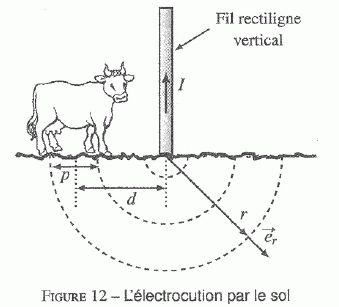
\includegraphics[width=0.4\linewidth]{electromag/electrostat/vache_foudre.png}
\end{center}

\begin{questions}

    \question Déterminer la densité de courant électrique $\vec{j}$ dans le sol.
    \question Rappeler l'expression de la loi d'ohm locale. Exprimer le champ électrique dans le sol et en déduire son potentiel $V(r)$ en le supposant nul à l'infini.
    \question Exprimer en fonction de $p$ et $d$ les potentiels au niveau des pattes avant et arrière de la vache. Quelle est la tension entre les pattes de la vache ?
    \question A quelle distance minimale $d_m$ du point d'impact est-elle en sécurité ?
    
    
    
\end{questions}

\paragraph{Données :} 
\begin{itemize}
    \item Foudre : $I=\SI{15}{kA}$
    \item Conductivité électrique du sol : $\gamma = \SI{1}{S/m}$
    \item Résistance de la vache : $R= \SI{30}{k\Omega}$
    \item Distance entre les pattes : $p=\SI{1.5}{m}$
    \item Courant létal pour une vache : $I_{max} = \SI{25}{mA}$
\end{itemize}

\end{exercise}

\begin{solution}
\begin{questions}

    \question $\vec j(r) = \frac{-I}{2\pi r^2} \vec{e}_r$
    \question $V(r) = \frac{-I}{2\pi \gamma  r} $
    \question $U = V(d+\frac{p}{2}) - V(d+\frac{p}{2}) \approx \frac{Ip}{2\pi \gamma d^2} $
    \question $d_m = \sqrt{\frac{Ip}{2\pi \gamma R I_{max} }}$
    
\end{questions}
\end{solution}


\section{Magnétostatique}
\begin{exercise}{Héliosphère solaire}{0}{Spé}
{Electromagnetisme, Magétostatique, Theoreme d'ampère, Plaque de courant}{bermudez}

\begin{questions}
    \questioncours Énoncé (succint) du théorème d'Ampère, version locale et intégrale. Comment passe-t-on de l'un à l'autre ?
    \uplevel{Le soleil possède des structures apparentées à de très fines couches de courant dans lesquelles sont dissipées l'énergie issue de la fusion nucléaire de l'étoile. On se propose de les modéliser par un plan en $z = 0$, infiniment fin, ayant un courant surfacique $\vec{j}_s = j_s \ve_x$.}
    \question Trouver l'expression du champ magnétique $\vec{B}$ engendré par le plan de courant.
    \question On considère maintenant la quantité $u = \dfrac{\vec{B}^2}{2\mu_0}$, qui a la dimension d'une énergie par unité de volume. Quelle est l'énergie engendrée par le plan de courant ?
\end{questions}

\end{exercise}


\begin{exercise}{Fil électrique}{0}{Spé}
{Electromagnetisme, Theoreme d'Ampère}{bermudez}

\begin{questions}
    \questioncours Énoncé (succint) du théorème d'Ampère, version locale et intégrale. Comment passe-t-on de l'un à l'autre ?
    \question On considère un cylindre de longueur infinie et de rayon $R$ parcouru par un courant $I$ uniformément réparti sur sa section. Trouver l'expression du champ magnétique $\vec{B}$ engendré par le fil, pour $r \leq R$ et $r \geq R$.
    \question On considère maintenant la quantité $u = \dfrac{\vec{B}^2}{2\mu_0}$, qui a la dimension d'une énergie par unité de volume. Quelle est l'énergie contenue dans un cylindre de rayon $r \leq R$ et de hauteur $H$ ? Même question pour $r \geq R$.
\end{questions}

\end{exercise}


\begin{exercise}{Bobine}{0}{Spé}
{Electromagnetisme, Theoreme d'Ampère}{bermudez}

\begin{questions}
    \questioncours Énoncé (succint) du théorème d'Ampère, version locale et intégrale. Comment passe-t-on de l'un à l'autre ?
    \uplevel{On considère un solénoïde modélisé comme un ensemble de boucles de courant de rayon $R$ parcourues d'un courant $I$ disposées sur un même axe de révolution avec une densité linéique $n_\ell$. On néglige les effets de bord.}
    \question Trouver l'expression du champ magnétique $\vec{B}$ engendré par le solénoïde, pour $r \leq R$ et $r \geq R$.
    
    \question Rappeler la définition de l'inductance $L$ en électronique en termes du champ magnétique $\vB$ et du courant $I$ et déduire de la question précédente l'inductance $L$ du solénoide. La calculer pour une bobine typique de TP $n_\ell = 10^4$ tours/m.
    \question On considère maintenant la quantité $u = \dfrac{\vec{B}^2}{2\mu_0}$, qui a la dimension d'une énergie par unité de volume. Quelle est l'énergie contenue dans un cylindre de rayon $r \leq R$ et de hauteur $H$ ? Même question pour $r \geq R$.
    \question Retrouver l'expression usuelle de l'énergie emmagasinée par une inductance.
\end{questions}

\paragraph{Données}

\begin{itemize}
    \item susceptibilité magnétique du vide $\mu_0 \simeq 4\pi \times 10^{-7}$ H$\cdot\text{m}^{-1}$.
\end{itemize}

\end{exercise}

\newpage

\begin{exercise}{Câble coaxial}{2}{Spé}
{Electromagnetisme, Theoreme d'Ampère}{bermudez}

\begin{questions}
    \questioncours Énoncé (succint) du théorème d'Ampère, version locale et intégrale. Comment passe-t-on de l'un à l'autre ?
    \uplevel{On considère un câble coaxial constitué de deux cylindres concentriques de longueur infinie et de rayons $R_1$ et $R_2 > R_1$. La région intérieure $r < R_1$, l'âme, est conductrice et est parcourue par un courant $I$ réparti uniformément sur sa section. La région $R_1 < r < R_2$, la gaine, est isolante et un courant $-I$ est réparti à sa surface en $r = R_2$.}
    \question  Trouver l'expression du champ magnétique $\vec{B}$ engendré par le courant $I$ dans la gaine, l'âme et à l'extérieur du câble coaxial.
    \question Rappeler la définition de l'inductance $L$ en électronique en termes du champ magnétique $\vB$ et du courant $I$ et déduire de la question précédente l'inductance de ligne $\Lambda$ (par unité de longueur du câble). La calculer pour un câble BNC usuel.
    \question On considère maintenant la quantité $u = \dfrac{\vec{B}^2}{2\mu_0}$, qui a la dimension d'une énergie par unité de volume. Quelle est l'énergie contenue dans  une longueur $H$ de câble coaxial ?
    \question Retrouver l'expression usuelle de l'énergie emmagasinée par une inductance.
\end{questions}

\paragraph{Données}

\begin{itemize}
    \item susceptibilité magnétique du vide $\mu_0 \simeq 4\pi \times 10^{-7}$ H$\cdot\text{m}^{-1}$.
\end{itemize}

\end{exercise}

\begin{solution}
    \begin{questions}
        \question ~
        \question Âme : $B(r) = \dfrac{\mu_0 I}{2\pi}\dfrac{r}{R_1^2}$, Gaine : $B(r) = \dfrac{\mu_0 I}{2\pi}\dfrac{1}{r}$, Extérieur : $B = 0$.
        \question $\cal{E}_\text{m} = \dfrac{\mu_0 I^2}{2\pi} L\qty(\dfrac{1}{4} + \ln\dfrac{R_2}{R_1})$
        \question D'où $\Lambda = \dfrac{\mu_0}{2\pi}\qty(\dfrac{1}{4} + \ln\dfrac{R_2}{R_1})$ \\
        AN : $R_1 = 2$ mm, $R_2 = 4$ mm, $\Lambda \sim 10^{-6}$ H$\cdot\text{m}^{-1}$.
    \end{questions}
\end{solution}
\begin{exercise}{Piège de Ioffe--Pritchard}{2}{Spé}
{Magnétostatique}{bermu, lelay}

\paragraph{Point méthode en électromagnétisme :}
\begin{itemize}
    \item à partir de la géométrie de problème, choisir le bon système de coordonnées ;
    \item utiliser les invariances du problème pour réduire le nombre de variables ;
    \item utiliser les symétries pour réduire le nombre de composantes ;
    \item identifier une surface fermée, un contour \emph{etc.} et appliquer le théorème intégral pertinent.
\end{itemize}


\begin{questions}
    \questioncours Exprimer le champ magnétique $\vB(\vr)$ d'un cylindre de rayon $R$ parcouru par un courant $I$, réparti volumiquement. On présentera les résultats d'électromagnétisme utiles.
    \question Justifier rapidement que l'on puisse écrire $\vB(\vr) = \rot(A(r)\ve_z)$, et trouver l'expression de $A(r)$ pour le champ précédent.
    \uplevel{On considère désormais le dispositif suivant : quatre fils conducteurs sont disposés aux sommets d'un carré de côté $2a$ et sont parcourus par des courants $+I$ et $-I$, alternativement.}
    \question Quelle est l'expression du potentiel vecteur $A(x, y)$ en un point $M$ d'un plan $(O, x, y)$ dont l'origine et les axes auront été judicieusement choisis ?
    \question Exprimer $A$ à l'ordre le plus bas pour $x$ et $y$ proches de l'origine.
    \question En déduire le champ magnétique $\vec{B}$ pour un point proche de l'origine. Son expression est-elle cohérente avec les invariances et les symétries de cette nouvelle configuration ? 
    \uplevel{On place dans ce champ un neutron de moment magnétique $\vec{m}$. À l'aide de techniques de pompage optique, il est possible de maintenir le moment magnétique du neutron dans la direction opposée de celle du champ.}
    
    \question Par analogie avec un dipôle électrique, donner l'énergie magnétique $E_m$ d'un tel neutron placé dans un champ $\vB$.
    
    \question Tracer la courbe $E_m(\rho)$ avec $\rho = \sqrt{x^2+y^2}$ pour le système étudié et commenter l'appellation "piège" de Ioffe pour ce dispositif.
    % \question On place dans ce champ un neutron de moment magnétique $\vec{m}$. Justifiez que le moment magnétique du neutron s'aligne avec celui du champ magnétique.
    % \question Quelle est la force appliquée par le champ magnétique sur le neutron ? En déduire la dynamique du neutron. Commenter l'appellation "piège" de Ioffe pour ce dispositif.
\end{questions}

\paragraph{Données :} 
% Rotationnel en coordonées cartésiennes
% $$\rot\vA = \qty(\pdv{A_z}{y} - \pdv{A_y}{z}) \ve_x
% + \qty(\pdv{A_x}{z} - \pdv{A_z}{x}) \ve_y
% + \qty(\pdv{A_y}{x} - \pdv{A_x}{y}) \ve_z$$ 
Rotationnel en coordonnées cylindrique
$$\rot\vA = \qty(\dfrac{1}{r}\pdv{A_z}{\theta} - \pdv{A_\theta}{z}) \ve_r
+ \qty(\pdv{A_r}{z} - \pdv{A_z}{r}) \ve_\theta
+ \qty(\dfrac{1}{r}\pdv{}{r} (r A_\theta) - \dfrac{1}{r}\pdv{A_r}{\theta}) \ve_z$$ 

\end{exercise}

\begin{solution}

\begin{questions}
    \questioncours $\vB(\vr) = \mu_o I/2\pi r \ve_\theta$
    \question On a $\vB(\vr) = \rot(A(r)\ve_z) = -\pdv{A}{r}\ve_\theta$ soit ici $A(r) = \mu_0 \frac{I}{2\pi}\ln(\frac{r}{R})$
    \uplevel{On considère désormais le dispositif suivant : quatre fils conducteurs sont disposés aux sommets d'un carré de côté $2a$ et sont parcourus par des courants $+I$ et $-I$, alternativement.}
    \question Les axes passent par les fils et le centre est au centre, les quatre distances aux fils sont $r_1 = \sqrt{x^2 + (a+y)^2}$, $r_2 = \sqrt{(a+x)^2 + y^2}$, $r_3 = \sqrt{x^2 + (a-y)^2}$, $r_4 = \sqrt{(a-x)^2 + y^2}$ et on a $$ A(x,y) =  \mu_0 \frac{I}{2\pi}\qty( \ln(\frac{r_1}{R}) - \ln(\frac{r_2}{R}) + \ln(\frac{r_3}{R}) - \ln(\frac{r_4}{R}) ) $$
    \question Attention il faut garder les termes d'ordre 2 c'est un peu degueulasse.
    \begin{align*}
        r_{1,3} & = a\sqrt{1 \pm 2\frac{y}{a} + \frac{x^2}{a^2} + \frac{y^2}{a^2}} \\
        &\approx a\qty(1 + \frac12\qty(\pm 2\frac{y}{a} + \frac{x^2}{a^2} + \frac{y^2}{a^2}) - \frac18\qty(2\frac{y}{a})^2) \\
        & = a\qty(1 \pm \frac{y}{a} + \frac12\frac{x^2}{a^2}) \\
        \ln(r_{1,3}) &= \ln\frac{a}{R} + \ln(1 \pm \frac{y}{a} + \frac12\frac{x^2}{a^2}) \\
        &\approx \ln\frac{a}{R} \pm \frac{y}{a} + \frac12\frac{x^2}{a^2} - \frac12\qty(\frac{y}{a})^2 \\
        &= \ln\frac{a}{R} \pm \frac{y}{a} + \frac12\frac{x^2-y^2}{a^2}
    \end{align*}
    et ainsi $r_{2,4}$ en échangeant $x$ par $y$ et vice versa.
    
    D'où
    \begin{align*}
        A(x,y) &=  \mu_0 \frac{I}{2\pi} \bigg(&& \\
        & &&+      \ln\frac{a}{R} + \frac{y}{a} + \frac12\frac{x^2-y^2}{a^2}\\ 
        & &&- \qty(\ln\frac{a}{R} + \frac{x}{a} - \frac12\frac{y^2-x^2}{a^2}) \\
        & &&+      \ln\frac{a}{R} - \frac{y}{a} + \frac12\frac{x^2-y^2}{a^2} \\
        & &&- \qty(\ln\frac{a}{R} - \frac{x}{a} + \frac12\frac{y^2-x^2}{a^2}) \\
        & &&\bigg)\\
        &=  \mu_0 \frac{I}{2\pi}\bigg(&& 2\frac{x^2-y^2}{a^2} \bigg) 
    \end{align*}
    
    \question On a $A(r) = \mu_0 \frac{I}{\pi}\frac{x^2-y^2}{a^2} $ et $B = (\partial_y A , -\partial_x A , 0) = -\mu_0 \frac{2I}{\pi a^2}(y, x, 0)$, $B$ ne dépend toujours pas de $z$.
    \uplevel{On place dans ce champ un neutron de moment magnétique $\vec{m}$. À l'aide de techniques de pompage optiques utilisant des faisceaux laser, il est possible de maintenir le moment magnétique du neutron dans la direction opposée de celle du champ.}
    
    \question $E_m = -\vec{m}\cdot \vB = m \abs{B}$ dans le cas où ils sont antiparallèle.
    
    \question On a $\abs{B} \propto \sqrt{x^2 +y^2}$ d'où $Em \propto \rho$ : on a bien un piège.
\end{questions}
\end{solution}

\begin{exercise}{Piège de Penning}{2}{Spé}
{Magnétostatique}{lelay}

On souhaite réaliser un champ électrostatique permettant de confiner des particules de charge $q > 0$ et de masse $m$ au voisinage d'un point $O$ dans le vide.

\begin{questions}
    \questioncours Équation de Maxwell--Gauss, équation de Poisson pour le potentiel.
    \uplevel{On envisage dans un premier temps de réaliser ce confinement en créant un champ électrostatique approprié. On admet qu'il est toujours possible de choisir un système d'axes $(Oxyz)$ pour que le développement limité du potentiel près de $O$ puisse s'écrire}
    $$
    V(x, y, z) = V_0 + a_1 x + a_2 y + a_3 z + b_1 x^2+ b_2y^2 + b_3z^2 + \order{\abs{\vr}^2}
    $$
    \question Comment doivent être les coefficients $b_i$ pour que le point $O$ soit un point d'équilibre ? Quid des $a_i$ et de $V_0$ ?
    \question Quelle équation locale est vérifiée par le potentiel, et qu'implique-t-elle quant aux coefficients $b_i$ ? Montrer qu'en conséquence de l'équation de Maxwell-Gauss, il est impossible de confiner une charge au voisinage d'un point en utilisant le seul champ électrique.
    \uplevel{On suppose qu'un arrive à réaliser à l'aide du système d'électrodes approprié le champ électrique $\vec{E}$ dérivant du potentiel $V$ si dessous}
    $$
    V(x, y, z) = -\frac{E_0}{2d}(x^2+y^2-2z^2)
    $$
    \question Une particule chargée positivement soumise à ce potentiel est confinée sur le plan $z = 0$. En déduire le signe de $E_0$. Qu'en est-il du mouvement de la particule dans le plan $xy$ ?
    \question On ajoute à l'installation un dispositif générant un champ $\vec{B} = B_0 \ve_z$ (Bonus : comment réaliser un tel champ expérimentalement ?). Établir l'équation différentielle vérifiée par $u = x+  iy$.
    \question Montrer que si le champ magnétique dépasse une valeur critique $B_c$, il est possible de confiner la particule.
    \question Déterminer $x(t)$ et $y(t)$ pour $B_0 \gg B_c$ en prenant comme condition initiale $\vec{OM} = x_0 \ve_x$ et $\vec{v}(0) = \vec{0}$. On fera apparaître deux pulsations caractéristiques.
    
\end{questions}

\paragraph{Données :} 
% Rotationnel en coordonées cartésiennes
% $$\rot\vA = \qty(\pdv{A_z}{y} - \pdv{A_y}{z}) \ve_x
% + \qty(\pdv{A_x}{z} - \pdv{A_z}{x}) \ve_y
% + \qty(\pdv{A_y}{x} - \pdv{A_x}{y}) \ve_z$$ 
Rotationnel en coordonnées cylindriques
$$\rot\vA = \qty(\dfrac{1}{r}\pdv{A_z}{\theta} - \pdv{A_\theta}{z}) \ve_r
+ \qty(\pdv{A_r}{z} - \pdv{A_z}{r}) \ve_\theta
+ \qty(\dfrac{1}{r}\pdv{}{r} (r A_\theta) - \dfrac{1}{r}\pdv{A_r}{\theta}) \ve_z$$ 

\end{exercise}

\begin{solution}
\begin{questions}
    \questioncours --
    \uplevel{On envisage dans un premier temps de réaliser ce confinement en créant un champ électrostatique approprié. On admet qu'il est toujours possible de choisir un système d'axes $(Oxyz)$ pour que le développement limité du potentiel près de $O$ puisse s'écrire}
    $$
    V(x, y, z) = V_0 + a_1 x + a_2 y + a_3 z + b_1 x^2+ b_2y^2 + b_3z^2 + \order{\abs{\vr}^2}
    $$
    \question Les $b_i$ doivent être positifs (Il faut un minimum global de potentiel), les $a_i$ doivent être nuls (0 est le minimum, pas un autre point) et $V_0$ peut importe, invariance de jauge le potentiel est défini à une constante près.
    \question Équation de Poisson, $\triangle V = 0$ donc au moins un des $b_i$ est positif : on ne peut pas faire de piège électrostatique.
    \uplevel{On suppose qu'un arrive à réaliser à l'aide du système d'électrodes approprié le champ électrique $\vec{E}$ dérivant du potentiel $V$ si dessous}
    $$
    V(x, y, z) = \frac{E_0}{2d}(x^2+y^2-2z^2)
    $$
    \question On a le long de l'axe $z$ $F_z = -eE_0 \frac{z}{d}$, qui est une force de rappel élastique ssi  $E_0 > 0$. Par contre en $z=0$ (dans le plan $xy$) on a $F_{xy} = qE = e -\grad_{xy} V = eE_0 \frac{x+y}{2d}$ : ça diverge exponentiellement !
    \question On a $$ \ddot u - i \omega_B \dot u - \frac{1}{\tau^2}u = 0 $$
    avec $\omega_B = \frac{qB}{m}$ la pulsation cyclotron et $\tau = \sqrt{md/q E_0}$ le temps typique d'éloignement de la particule.
    \question Le déterminant de l'équation caractéristique est $(-i\omega_b)^2 - 4(-1/\tau^2) = 4/\tau^2 - \omega_B^2$ qui est négatif (racine imaginaires pures, solutions purement oscillantes donc système stable) pour $\omega_B > 2/\tau$ soit $B_0 > 2\sqrt{E_0 m/ dq}$
    \question Les pulsations d'oscillations sont 
    \begin{align*}
        \omega_\pm &= \frac{\omega_B}{2}\qty(1 + \sqrt{1 - \frac{1}{\tau^2\omega_B^2}}) \\
        &\approx \omega_B \qqtext{ou bien} 1/2\tau^2\omega_B
    \end{align*} 
    soit une pulsation ra[ide et une pulsation lente.
    
\end{questions}
\end{solution}


\section{Equations de Maxwell}
\begin{exercise}{Divergence en cylindrique}{0}{Spé}
{Electromagnetisme, Conservation de la charge}{bermu}

\begin{questions}
    \questioncours Donner les 4 équations de Maxwell avec sources sous forme locale et en déduire l'équation de conservation de la charge. \\
    On notera $\vec{j}(\vr,t)$ et $\rho(\vr,t)$ les densités de courant et de charge.
    
    \uplevel{On considère un tube cylindrique, de hauteur $h$, de rayon $r$ et d'épaisseur $dr$. Ce tube reçoit sur sa surface intérieure un flux de charge uniforme, quantifié par le vecteur densité de courant $\vec{j}(r, \theta, z, t) = j(r, t)\vec{e_r}$, et perd depuis sa surface extérieure un flux de charge, donné par $j(r+dr, t) \vec{e_r}$. On note $Q(t)$ sa charge totale et $\rho(r, t)$ sa densité volumique de charge, supposée uniforme dans le tube.}
    
    \uplevel{On considère une électrode cylindrique de rayon $a$ et de hauteur $H \gg a$ qui émet un courant radial~$I(t)$.}
    
    \question Quelles sont les symétries de $\rho$ et $\vec{j}$ ?
    
    \question On étudie la conservation de la charge dans le cylindre. Effectuer un bilan de charges entre $t$ et $t + \dd{t}$, $r$ et $r + \dd{r}$ et retrouver l'équation de la conservation de la charge précédemment obtenue.

    \question En déduire l'expression de la divergence du champ $\vec{j}$ en coordonnées cylindriques.

\end{questions}

\end{exercise}

% Niveau :      PC
% Discipline :  Electromagnétisme
%Mots clés :    Equations de Maxwell, Drude

\begin{exercise}{Relaxation des charges dans un métal}{2}{Spé}
{\'Equations de Maxwell, Temps de Maxwell,Plasma résistif}{bermu}

On considère un plasma conducteur constitué d'un gaz neutre d'ions et d'électrons de densité de charges $\rho$ et de conductivité électrique $\sigma$. On considérera les ions immobiles.

\begin{questions}
    \questioncours Établir l'équation de la conservation de la charge à partir des équations de Maxwell.
    \question Montrez que la densité de charges créé un champ électrique $\vE$, induisant lui-même un courant électrique $\vJ$.
    \question \'Etablir l'équation régissant $\rho$. On fera apparaître un temps caractéristique $\tau_\textsc{m}$, le temps de Maxwell, dont on donnera une interprétation physique.
    \question Calculer le temps de Maxwell le cuivre, $\sigma = 6\times 10^8$ $\Omega^{-1}\cdot\text{m}^{-1}$. \`A quelle condition peut-on considérer que les charges dans circuit électrique sont toutes relaxées ?
\end{questions}

\paragraph{Données :}
\begin{itemize}
    \item permittivité du vide $\varepsilon_0 = 8,854\times 10^{-12}$ F$\cdot$m$^{-1}$.
\end{itemize}
\end{exercise}

\begin{solution}
\begin{questions}
    \question $\pdv{\rho}{t} + \div\vJ = 0$
    \question $\div \vE = \dfrac{1}{\sigma}\div\vJ =\dfrac{\rho}{\ep_0}$
    \question $\pdv{\rho}{t} + \dfrac{1}{\tau_\textsc{m}} \rho = 0$ avec $\tau_\textsc{m} = \dfrac{\ep_0}{\sigma}$
    \question $\tau_\textsc{m} = 1 \times 10^{-20}$ s. On doit donc avoir $f < 10^{20}$ Hz : toujours vrai !
\end{questions}
\end{solution}


% Niveau :      PC
% Discipline :  Electromagnétisme
%Mots clés :    Equations de Maxwell, Drude

\begin{exercise}{\'Ecrantage magnétique \textbullet\ Effet Meissner}{2}{Spé}
{\'Equations de Maxwell,Plasma inertiel}{bermu}

On considère un plasma constitué d'un gaz neutre d'ions et d'électrons de densité $n$. On considérera les ions immobiles. On impose dans une région $x<0$ de ce gaz un champ magnétique homogène $\vB_0(t) = B_0(t) \ve_z$. On étudie le régime de relaxation des courants dans $x>0$.

\begin{questions}
    \question Montrez qu'un champ $\vB$ induit un champ $\vE$. On supposera que $\vB = B(t)\ve_z$ et $\vE = E\ve_y$ (le justifier). Donner la relation (1) entre $E$ et $B$.
    \question Montrez que par conséquent, les électrons se mettent en mouvement et établir une équation (2) entre la densité de courant $J$ et le champ $E$.
    \question Montrez que le courant $J$ rétroagit lui-même sur $B$ et donner la relation (3) entre les deux.
    \question En déduire l'équation vérifiée par $E$. On fera apparaître une longueur caractéristique $\ell_\text{p}$, la longueur de London.
    \question Au vu des conditions aux limites, résoudre l'équation pour $B$, puis $E$, puis $J$ et en déduire une interprétation de la longueur de London.
    \question Calculer la longeur de London pour un plasma de densité $n = 10^{23}$ m$^{-3}$.
\end{questions}

\paragraph{Données :}
\begin{itemize}
    \item charge élémentaire $e = 1,602\times 10^{-19}$ C,
    \item masse le l'électron $m_e = 9,109\times 10^{-31}$ kg,
    \item pereabilité du vide $\mu_0 = 1,26 \times 10^{-6}$ $H\cdot$m$^{-1}$.
\end{itemize}
\end{exercise}

\begin{solution}
\begin{questions}
    \question Maxwell Faraday (1) $\pdv{E}{x} = -\pdv{B}{t}$
    \question Newton PFD (2) $\pdv{J}{t} = -\dfrac{ne^2}{m_e} E$
    \question Maxwell Ampère (3) $\pdv{B}{x} = -\mu_0 J$ (on vire le courant de déplacement de l'ordre de $v/c$).
    \question D'où $\pdv[2]{E}{x} = \ell_\text{p}^{-2}E$, $\ell_\text{p} = \dfrac{m_e}{\mu_0 e^2} = \dfrac{c}{\omega_\text{p}}$.
    \question $B(x,t) = B_0(t) e^{-x/\ell_\text{p}}$, $E(x,t) = \ell_\text{p} B'_0(t) e^{-x/\ell_\text{p}}$, $J = J_0 e^{-x/\ell_\text{p}}$.
\end{questions}
\end{solution}






% Niveau :      PC
% Discipline :  Electromagnétisme
%Mots clés :    Equations de Maxwell, Drude

\begin{exercise}{Lampe à plasma}{3}{Spé}
{\'Equations de Maxwell,\'Equation de conservation,Statique des fluides}{bermu}

\begin{questions}
    \questioncours Rappeler l'expression de la conductivité $\sigma$ d'un nuage d'électrons du modèle de Drude en fonction de sa densité $n$ et la fréquence de collision des électrons $\nu_\text{c}$, et d'autres données nécessaires. \\
    Expliciter la relation entre la vitesse $\vv$ des électrons et le potentiel $V(\vr)$ dans lequel ils se trouvent.
\begin{EnvUplevel}
Afin de modéliser une décharge électrique près d'une électrode d'une lampe à plasma, considérons un gaz d'atomes qui s'ionise. On considère alors la densité d'électrons $n_e(\vr)$ et d'ions $n_i(r)$ autour de la boule.

Le nuage électronique créé un champ de pression $p(\vr)$ et un champ électrique $V(\vr)$ à cause des charges.
\end{EnvUplevel}
    \question Considérant que le gaz électronique est à l'équilibre hydrostatique à la température $T$ et que son équation d'état est celle d'un gaz parfait, donner une relation entre la densité du gaz $n_e(\vr)$, le potentiel électrique $V(r)$ et la température $T$. \\
    Cette loi vous rappelle-t-elle quelque chose ? Discuter cette hypothèse.
\uplevel{On modélise la boule plasma comme une électrode quasi plane en $z=0$ portée au potentiel $V_0 = 10$~kV et un gaz d'ions et d'électrons en $z>0$ supposé quasi neutre $n_i = n_e = n$.}
    \question Considérant qu'à chaque collision avec un atome, un électron expulse $\alpha$ électrons et en notant son libre parcours moyen $\ell$ et l'énergie de première ionisation des atomes $V_\text{ion}$ (en volts), estimer par un raisonnement de votre choix $\alpha$.
    \question Justifier que le taux d'ionisation peut s'écrire $\alpha\nu_\text{c}n$ et déduire de la relation de conservation des électrons un lien entre $\vv$ et $n$.
    \question Déduire des questions précédentes l'équation de Schottky
    $$\qty(\grad^2 - {\ell_\textsc{s}}^{-2})n = 0,$$
    en exprimant la longueur de Schottky $\ell_\textsc{s}$ en fonction des données du problème et la vitesse
    $$c_\textsc{s} = \sqrt{\dfrac{k_\textsc{b}T}{m_e}}.$$
    Interpréter physiquement $\ell_\textsc{s}$ et $c_\textsc{s}$.
    \question Quelle est l'équation régissant $V(\vr)$ ?
    \question Résoudre et tracer les profils de potentiel $V(\vr)$, de densité $n(\vr)$ et de vitesse $\vv(\vr)$ ?
    \question Montrez que les particules passent le mur du son. Interpréter. Considérant que la décharge électrique se dissipe à ce moment là, estimer la taille de la décharge électrique.
\end{questions}

\paragraph{Données :}
\begin{itemize}
    \item charge élémentaire $e = 1,602\times 10^{-19}$ C,
    \item masse le l'électron $m_e = 9,109\times 10^{-31}$ kg,
    \item permittivité du vide $\varepsilon_0 = 8,854\times 10^{-12}$ F$\cdot$m$^{-1}$,
    \item vitesse de la lumière dans le vide $c = 2,998 \times 10^8$ m$\cdot$s$^{-1}$,
    \item constante de Boltzmann $k_\textsc{b} = 1,381\times 10^{-23}$ J$\cdot$K$^{-1}$,
    \item Dans une décharge électrique : $T = 10 000$ K, $n = 10^{23}$ m$^{-3}$.
\end{itemize}
\end{exercise}

\section{Ondes électromagnétiques}
\begin{exercise}{Onde électromagnétique}{0}{Spé}
{Ondes électromagnétiques,Vide}{lelay}

On étudie la propagation d'une onde électromagnétique dans le vide dont le champ électrique correspondant est de la forme $\vec{E} = E_0\cos(\omega t - kz)\vec{u}_x$.
\begin{questions}
    \questioncours Rappeler les équations aux dérivées partielles auxquelles sont soumis les champs électriques et magnétiques dans le vide.
    \question Quelle est la direction, le sens et la vitesse de propagation de cette onde ? Quel type d'onde est-ce ? 
    \question Exprimer le vecteur d'ondes $\vec{k}$, le champ magnétique $\vec{B}$ et le vecteur de Poynting associés à l'onde.
    \question On suppose que cette onde rayonne à travers une surface effective $S = 4$ mm$^2$ une puissance moyenne $P = 10$ mW (valeur typique pour un laser de classe III.b). Calculer les amplitudes $E_0$ ey $B_0$ des champs électriques et magnétiques.
    \question La longueur d'onde de ce rayonnement est de 632 nm dans l'air. Dans quel domaine du spectre électromagnétique se situe cette onde ?
    \question Donner la fréquence correspondante en THz.
\end{questions}

\end{exercise}

\begin{solution}

\begin{questions}
    \questioncours Eqn de Mxl sans les sources
    \question direction $z$, sens propageant ($+z$), vitesse de propagation $c$ (on est dans le vide). OPPH (onde propageante plane harmonique) polarisée rectilignement
    \question $\vec{k} = \frac{\omega}{c}\vec{u}_z$, $\vec{B} = \frac{E_0}{c}\cos(\omega t - kz) \vec{u}_y$, vecteur de Poyting $\vec{\Pi} = EB/\mu_0 = E_0^2/(c\mu_0) \cos^2(\omega t - kz)$
    \question $\ev{\vec{\Pi}} = \frac12 \frac{E_0^2}{c\mu_0} = 2.5$ mW/mm$^2$. D'où $E_0$ et $B_0  =E_0 / c$
    \question Visible (rouge)
    \question $\nu = v_\phi / \lambda$, $v_\phi = c/n \approx c$ car $n_\text{air} \approx 1$
\end{questions}
\end{solution}
\begin{exercise}{Vitesse de phase, vitesse de groupe}{1}{Spé}
{Ondes électromagnétiques}{lelay}

On étudie la propagation d'une onde électromagnétique dans un milieu transparent d'indice $n$ régit par la loi de Cauchy : 
$$
n = A + \frac{B}{\lambda^2}
$$
où $A$ et $B$ sont des constantes dépendant du matériau.
\begin{questions}
    \questioncours Donner la définition de la vitesse de phase et de la vitesse de groupe ainsi que leur interprétation.
    \question Quelle est la vitesse de phase de l'onde considérée ?
    \question Quelle est sa vitesse de groupe $v_g$ ?
    \question En considérant que $B/\lambda^2 \ll A$, exprimer $v_g$ au premier ordre non nul en $k$
    \question Comment varie cette vitesse avec la fréquence de la lumière étudiée ? Comment évolue une impulsion lumineuse initialement blanche au fur et à mesure qu'elle progresse dans le milieu ?
\end{questions}

\end{exercise}

\begin{solution}

\begin{questions}
    \questioncours --
    \question $v_\phi = c/n$
    \question $v_g=\dv{\omega}{k}$ mais $\omega = ck/n$ d'où $c\dv{k/n}{k} = c/n\qty(1 -k \dv{n}{k}) = c/n\qty(1-k^2\frac{B}{2\pi^2 n})$
    \question $ v_g= c/A\qty(1-k^2\frac{3B}{4\pi^2 A})$
    \question augmente avec lambda, diminue avec $f$. Le rouge va plus vite et va à l'avant, le bleu plus lentement et va à l'arrière, le paquet d'onde s'étale et est soumis à de la dispersion chromatique
\end{questions}
\end{solution}
% Rayonnement dipolaire (MP)
\begin{exercise}{Antenne}{1}{Spé}
{Rayonnement dipolaire}{lelay}

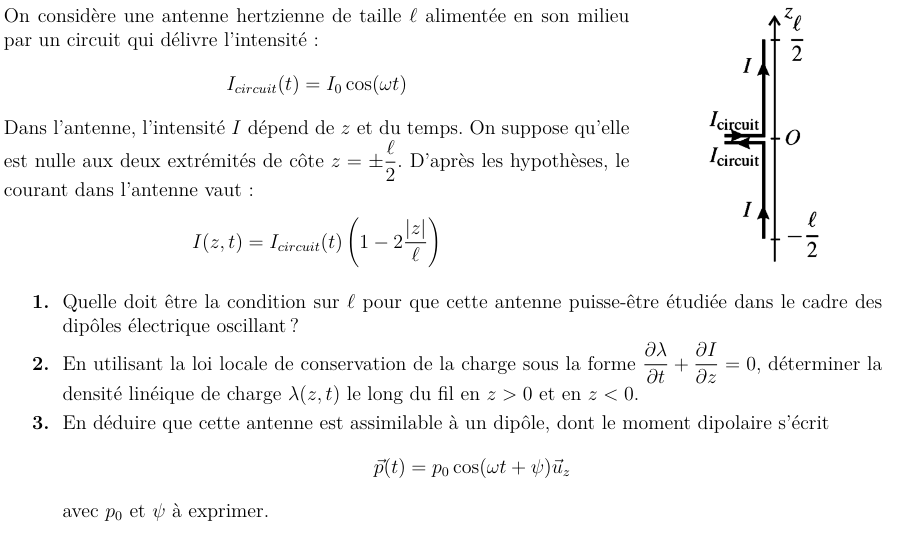
\includegraphics[width=\textwidth]{electromag/ondesEM/antenne.png}

\end{exercise}

% \begin{solution}
% \begin{questions}
%     \questioncours ?!
% \end{questions}
% \end{solution}

\begin{exercise}{Dipôle magnétique oscillant}{2}{Spé}
{Rayonnement dipolaire}{lelay}

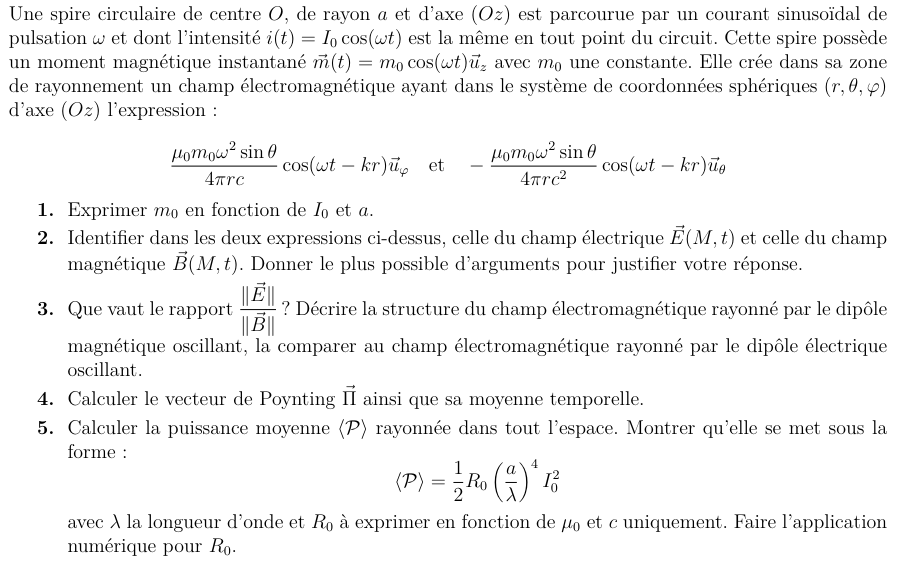
\includegraphics[width=\textwidth]{electromag/ondesEM/rayonnementdipolairespire.png}

\end{exercise}

% \begin{solution}
% \begin{questions}
%     \questioncours ?!
% \end{questions}
% \end{solution}

% Guidé (MP)
\begin{exercise}{Protection d'un four à micro-ondes}{2}{Spé}
{Ondes électromagnétiques,Guide d'ondes,Réflection métallique}{lelay}

On considère une plaque métallique d'épaisseur $d$ et de normale $\ve_z$ dans le vide. Cette plaque est percée d'une ouverture carrée de côté $a$. Un OPPH électromagnétique polarisée selon $\ve_x$ arrive depuis $-\infty$ sur la plaque.
\begin{questions}
    \questioncours Propriétés du conducteur parfait, conditions aux limites des champs électriques et magnétiques.
    \question On cherche à déterminer la champ $\vec{E}$ se propageant dans l'ouverture. Justifier qu'on le cherche sous la forme
    $$
    \vec{E}(x, y, z) = E_0 f(x,y) e^{i(\omega t - k z)} \ve_x
    $$
    \begin{parts}
        \part Quelle est la dépendance de $f$ en $x$ ?
        \part Quelle est l'équation de propagation vérifiée par $\vec{E}$ ? En déduire l'équation différentielle vérifiée par $f$.
        \part Quelles sont les conditions aux limites pour $\vec{E}$ ?
        \part En déduire que les fonctions $f$ possibles appartiennent à une famille de fonctions $(f_n)$ indexées par un entier $n$.
    \end{parts}
    \uplevel{On considère par la suite le cas $n=1$.}
    \question Exprimer le champ magnétique dans l'ouverture.
    \question À quelle condition sur $a$ et $f$ l'onde se propage-t-elle ?
    \question Que se passe-t-il si cette condition n'est pas respectée ? On introduira une longueur caractéristique pertinente $\delta$.
    \question Estimer l'épaisseur de la plaque métallique accolée à la fenêtre d'un micro-ondes ($f = 2.45$ GHz).
\end{questions}

\end{exercise}

\begin{solution}

\begin{questions}
    \questioncours $E=B=J=\rho=0$ condition de passage, $E_\perp = 0$.
    \question 
    \begin{parts}
        \part $\div\vE=0$ donc $\pdv{f}{x}=0$.
        \part $\pdv[2]{\vE}{t} = c^2\grad^2\vE$ donc $f'' + (\omega^2/c^2 - k^2)f$.
        \part $E_\perp = 0$, $f(y=0)=f(y=a)=0$.
        \part $f_n(y) = f_{n0} \sin(2\pi n y/ a)$
    \end{parts}
    \question $\rot\vE = -\pdv{\vB}{t}$ D'où $ \vB = -E_0/\omega \mqty(0 \\ k \sin(2\pi y/a) \\ 2i\pi/a\cos(2\pi y/a))e^{i\omega t -kz}$
    \question On a $f^2/c^2 = \lambda^{-2} + a^{-2}$, donc il faut $f^2/c^2 > a^{-2}$ soit $a > c/f$.
    \question Si ce n'est pas respecté, $k^2 = \omega^2/c^2 - 4\pi^2/a^2$ soit donc $k = i\sqrt{4\pi^2/a^2 - \omega^2/c^2} = 1/\delta$...
    \question $a = 122$ $\mu$m.
\end{questions}

\end{solution}

% Plasma et rflexion métallique
\begin{exercise}{Effet de peau}{2}{Spé}
{\'Equations de Maxwell,Diffusion magnétique,Longeur de Kelvin,Plasma résistif,Rélfexion métallique }{bermu}

On considère un plasma conducteur constitué d'un gaz neutre d'ions et d'électrons de densité $n$ et de conductivité électrique $\sigma$. On considérera les ions immobiles. On impose dans une région $x<0$ de ce gaz un champ magnétique homogène oscillant $\vB_0(t) = B_0 \cos{\omega t} \ve_z$. On étudie le régime de relaxation des courants dans $x>0$.

\begin{questions}
    \question Montrez qu'un champ $\vB$ induit un champ $\vE$. On supposera que $\vB = B(t)\ve_z$ et $\vE = E\ve_y$ (le justifier). Donner la relation (1) entre $E$ et $B$.
    \question Montrez que par conséquent, un courant $J$ se créé et donner la relation (2) entre la densité de courant $J$ et le champ $E$.
    \question Montrez que le courant $J$ rétroagit lui-même sur $B$ et donner la relation (3) entre les deux.
    \question En déduire l'équation vérifiée par $B$. On fera apparaître la quantité $\eta = \dfrac{1}{\mu_0\sigma}$ dont on donnera un sens physique. Quelle est la nature de cette équation ?
    \question Au vu des conditions aux limites, résoudre l'équation pour $B$, puis $E$, puis $J$. On fera apparaître une longueur caractéristique $\ell_\textsc{k}$, la longueur de Kelvin, dont on donnera une interprétation.
    \question \`A quelle condition peut-on considérer que les courants dans un circuit de taille $L$ sont tous relaxés ?
\end{questions}

\paragraph{Données :}
\begin{itemize}
    \item charge élémentaire $e = 1,602\times 10^{-19}$ C,
    \item masse le l'électron $m_e = 9,109\times 10^{-31}$ kg,
    \item permeabilité du vide $\mu_0 = 1,26 \times 10^{-6}$ $H\cdot$m$^{-1}$,
    \item conductivité du cuivre $\sigma = 6\times 10^8$ $\omega^{-1}\cdot\text{m}^{-1}$.
\end{itemize}
\end{exercise}

\begin{solution}
\begin{questions}
    \question Maxwell Faraday (1) $\pdv{E}{x} = -\pdv{B}{t}$
    \question Loi d'Ohm (2) $J = \sigma E$
    \question Maxwell Ampère (3) $\pdv{B}{x} = -\mu_0 J$ (on vire le courant de déplacement de l'ordre de $v/c$).
    \question D'où $\pdv[2]{E}{xt} = \ell_\text{p}^{-2}E$, $\ell_\text{p} = \dfrac{m_e}{\mu_0 e^2} = \dfrac{c}{\omega_\text{p}}$.
    \question $B(x,t) = B_0(t) e^{-x/\ell_\text{p}}$, $E(x,t) = \ell_\text{p} B'_0(t) e^{-x/\ell_\text{p}}$, $J = J_0 e^{-x/\ell_\text{p}}$.
\end{questions}
\end{solution}

\begin{exercise}{Onde électromagnétique longitudinale}{2}{Spé}
{Ondes électromagnétiques,Plasma inertiel}{lelay}

On étudie la propagation dans un plasma peu dense d'une onde électromagnétique dont le champ électrique s'exprime $\vec{E} = \vec{E_0}\cos(\omega t - \vec{k}\cdot\vec{r})$.
\begin{questions}
    \questioncours Structure d'une onde électromagnétique dans le vide.
    \question Établir l'équation du mouvement d'un électron, de masse $m_e$ et associé à la densité $n_e$, en faisant les approximations qui sembleront nécessaires.

    \question Que dire du mouvement des ions ?
    
    \question Montrer que la conductivité $\sigma$ du plasma pour cette onde est complexe et en donner une expression.

    \uplevel{On considère que la densité locale du plasma $\rho$ est non nulle.}
    
    \question En utilisant l'équation locale de conservation de la charge, établir une nouvelle expression de la conductivité $\sigma$.
    
    \question En déduire la pulsation de l'onde obtenue.
    
    \question Montrer que le champ magnétique $\vec{B}$ associé à cette onde est nul dans tout le plasma. En déduire la direction de $\vec{k}$. Quel type d'onde est-ce ?
\end{questions}

\end{exercise}

\begin{solution}

\begin{questions}
    \questioncours triedre EBk direct
    \question $m \dot{v} = -e E$. force de lorentz magnetique negligeable

    \question Ions lents osef
    
    \question $\sigma = e n_e v$ d'où $\sigma = -in_e e^2/m\omega$

    \uplevel{On considère que la densité locale du mplasma $\rho$ est non nulle.}
    
    \question $\dot \rho = i\omega \rho$ et $\div j = \sigma \div E = \sigma \rho/\epsilon_0$ d'où $(i\omega + \sigma/\epsilon_0)\rho = 0$. $\rho \neq 0$ donc $\sigma = -i\omega \epsilon_0$
    
    \question $\omega = \omega_p = \sqrt{\frac{ne^2}{m\epsilon_0}}$
    
    \question $\rot B = 0$ or $\div B = 0$ donc $B = 0$. maxwell-faraday donne $E$ colineaire a $k$, d'où une onde LONGITUDINALE
\end{questions}
\end{solution}

% Milieux complexes
% Niveau :      PC
% Discipline :  Electromagnétisme
%Mots clés :    Equations de Maxwell, Drude

\begin{exercise}{Modèle de Drude pour les isolants}{2}{Spé}
{Ondes électromagnétiques,Plasma,Diélectrique}{bermu}

\paragraph{Rappel :} le modèle de Drude décrit la dynamique des électrons dans un champ électrique $\vE$ de la manière suivante
$$m\dv[2]{\vv}{t} = q\vE - m\gamma\pdv{\vr}{t}.$$
où $\vr$ est la position de la particule, $m$ sa masse, $q$ sa charge.
\begin{questions}
    \questioncours Rappeler les conditions du modèle de Drude et la relation de dispersion des ondes dans un conducteur décrit par ce modèle.\\
    On introduira et estimera un ordre de grandeur de la fréquence $\gamma$, la densité du plasma $n$, la pulsation plasma $\omega_\textsc{p}$ et de la conductivité $\sigma$.
\begin{EnvUplevel}
    Afin de généraliser ce modèle pour un isolant, Drude a également proposé le modèle suivant
    $$m\dv[2]{\vv}{t} = q\vE -m{\omega_0}^2\vr - m\gamma\pdv{\vr}{t}.$$
\end{EnvUplevel}
    \question Rappeler ce qu'est un diélectrique. Quelle différence y a-t-il avec un conducteur ? En déduire le sens du terme en $\omega_0$. \\
    Pour un diélectrique $\omega_0$ est dans le domaine visible.
    \question Déduire du modèle précédent la polarisabilité $\alpha$ du diélectrique, telle que le moment dipolaire
    $$\vp = \alpha\vE.$$
    Quelle est l'unité de $\alpha$ ?
    \question En utilisant le fait que la perméabilité $\varepsilon(\omega)$ d'un diélectrique s'écrit
    $$\varepsilon(\omega) = 1 + n\alpha = \dfrac{k^2c^2}{\omega^2},$$
    déduire de la question précédente la relation de dispersion des électrons.
    \question Montrer que pour $\gamma$ faible (on dira devant quoi et on vérifiera si cela est vrai) que la relation de dispersion des ondes peut s'écrire
    $$k^2 = \dfrac{\omega^2}{c^2}\:\dfrac{\omega^2 - {\omega_\infty}^2}{\omega^2 - {\omega_0}^2},$$
    avec $\omega_\infty$ dont on donnera l'expression et le sens physique.
    \question Tracer la relation de dispersion et montrer qu'il existe une bande interdite en fréquence et comparer au cas du simple conducteur.
    \question Peut-on construire une cage de Faraday avec une bâche en plastique ?
\end{questions}

\paragraph{Données :}
\begin{itemize}
    \item charge élémentaire $e = 1,602\times 10^{-19}$ C,
    \item masse le l'électron $m_e = 9,109\times 10^{-31}$ kg,
    \item vitesse de la lumière dans le vide $c = 2,998 \times 10^8$ m$\cdot$s$^{-1}$,
    \item permittivité du vide $\varepsilon_0 = 8,854\times 10^{-12}$ F$\cdot$m$^{-1}$,
\end{itemize}
\end{exercise}
\begin{exercise}{Lame quart d'onde}{2}{Spé}
{Ondes électromagnétiques,Biréfringence}{lelay}

On considère une lame biréfringente d'épaisseur $e$ et de normale $\ve_z$. Biréfringente signifie que la propagation selon l'axe $Ox$ est caractérisée par un indice $n_x$ et la propagation selon l'axe $Oy$ par un indice $n_y$. La lame est transparente et non absorbante. Les axes $Ox$ et $Oy$ sont appelés \emph{lignes neutres} de la lame.
\begin{questions}
    \questioncours Équation de propagation de la lumière, notion d'indice optique.
    \question On suppose $n_x < n_y$. Expliquer pourquoi la ligne neutre $Ox$ est appelée \textit{axe rapide} alors que $Oy$ est appelée \textit{axe lent}.
    \question À l'entrée de la lame, en $z = 0$, on considère une onde électromagnétique incidente sous la forme d'une OPPH de longueur d'onde $\lambda_0$ dans le vide dont le champ électrique s'écrit en $z=0$
    $$
    \vec{E} = \vec{E}_0\cos(\omega t)
    $$
    Une fois dans la lame, quelle est l'équation différentielle vérifiée par chacune des composantes du champ électrique ?
    \question Donner la forme de $\vec{E}$ en sortie de la lame, en utilisant la notation $\bar{n} = n_y+n_x$ et $\Delta n = n_y-n_x$.
    \question Exprimer $\vec{E}_0$ si l'onde incidente est polarisée selon $\ve_x$. Caractériser l'état de polarisation en sortie de la lame.
    \uplevel{On se place maintenant dans le cas où l'épaisseur $e$ de la lame vérifie $\frac{\omega}{c}(n_y-n_x)e = \frac{\pi}{2}$.}
    \question Exprimer $e$ en fonction de $\lambda_0$ et $\Delta n$. Justifier l'appellation \textit{lame quart d'onde} pour ce type d'objets.
    \question On considère le cas $\vec{E}_0 = E_0 \qty(\frac{\ve_x}{\sqrt{2}}+\frac{\ve_y}{\sqrt{2}})$. Quelle est l'état de polarisation de la lame en entrée ? Faire un schéma. Que devient cet état en sortie de lame ?
    \question L'onde incidente est maintenant polarisée circulairement. Comment est alors $\vec{E}_0$ ? Que devient la polarisation en sortie de lame ?
    \question On place, sur un miroir plan l'ensemble constitué d'un polarisateur rectiligne P et d'une lame quart d'onde Q. L'axe du polariseur est  selon une bissectrice des lignes neutres de Q. Qu'observe-t-on à travers l'ensemble P+Q+miroir ?
\end{questions}

\end{exercise}
\begin{exercise}{Loi de Biot}{3}{Spé}
{Ondes électromagnétiques,Polarisation rotatoire}{lelay}

On considère la propagation d'une OPPH électromagnétique dans un milieu optiquement actif occupant l'espace $z > 0$. Dans ce milieu, les ondes se propagent différemment en fonction de leur polarisation, ici les ondes polarisées circulairement gauches et droites se propagent avec des indices $n_g$ et $n_d$. On considère une OPPH se propageant dans la direction $Oz$, polarisée rectilignement selon $\ve_x$ en $z=0$.
\begin{questions}
    \questioncours Équation de propagation de la lumière, polarisation.
    \question Montrer que l'onde incidente, dans le vide ($z < 0$) peut s'écrire comme la superposition de deux ondes polarisées circulairement gauche et droite.
    \question Quelle est la polarisation de l'onde en $z$ quelconque, $z \geq 0$ ?
    \question Une substance est dite \textit{dextrogyre} si une onde initialement polarisée vers le haut (pour un observateur en face d'elle) tourne `vers la droite' d'un angle $\theta >0$, si elle tourne dans l'autre sens on dit que la substance est \textit{lévogyre}. Comment se traduit la différence entre ces deux milieux en fonction du signe de $\Delta n$ ?
    \question En s'inspirant de la loi de Beer-Lambert, donner la forme de la loi de Biot qui donne l'angle de rotation du plan de polarisation d'une onde lumineuse à travers une solution en fonction de la longueur de la cuve $\ell$, de la concentration de la solution $c$ et du pouvoir rotatoire spécifique du composé $[\alpha]$, dont on précisera l'unité.
\end{questions}

\end{exercise}

%WTF
\begin{exercise}{Pression de radiation}{2}{Spé}
{Ondes électromagnétiques}{lelay}

On considère une onde plane, monochromatique de fréquence $\nu$ se propageant dans la direction des $z$ croissant et dont le champ électrique s'exprime $\vec{E} = E_0\cos(\omega t - kz)\vec{u}_x$.
\begin{questions}
    \questioncours Rappeler l'équation aux dérivées partielles vérifiée par les champs $\vec{E}$ et $\vec{B}$ correspondant à cette onde.
    \question exprimer le champ magnétique associé à cette onde, puis son vecteur de Poynting.
    \question Exprimer l'éclairement $\mathcal{E}$, c'est-à-dire la puissance surfacique moyenne de l'onde dans la direction perpendiculaire à la propagation, en fonction de $E_0$, $c$ et $E_0$. 

    \uplevel{D'après le principe de la dualité onde-particule de la physique quantique, on peut aussi considérer cette onde comme un flux de photons individuels.}
    
    \question Quelle serait alors l'énergie de chacun de ces photons ?
    \question En déduire le flux surfacique de photons $\phi$ (nombre de photons traversant une surface du plan $x,y$ par unité de temps et de surface) correspondant à cette onde.
    \question Quel est la quantité de mouvement porté par chacun des photons ? En déduire le flux de quantité de mouvement surfacique de l'onde.
    
    \uplevel{On suppose que cette onde arrive sur un objet de masse $m$ présentant une surface $S$, orthogonale à la direction de propagation.}
    
    \question Donner l'énergie et la quantité de mouvement fournies par unité de temps à l'objet dans les cas suivants :
    \begin{parts}
        \part La surface est noire (absorbant parfaitement le rayonnement électromagnétique)
        \part La surface est un miroir
        \part La surface est blanche
    \end{parts}
    \question Sachant que la puissance surfacique reçue au niveau de la Terre est de 1.2 kW/m$^2$, donner la puissance lumineuse du Soleil $P_0$
    \question Quelle est la force de pression de radiation subie par une sphère absorbante (noire) de rayon $a$ située à une distance $r$ du Soleil ?
    \question Comparer cette force à la gravité pour les cas suivants
    \begin{parts}
        \part Une météorite ($a = 1$ m, $m = 10$ tonnes)
        \part Un grain de poussière stellaire ($a = 0.1$ $\mu$m, $m = 10^{-17}$ kg)
    \end{parts}
\end{questions}

\end{exercise}

\begin{solution}

\begin{questions}
    \questioncours Equation de d'alembert
    \question $B_0 = E_0/c$, $\Pi =E_0 B_)0/\mu_0 \cos^2(\omega t - kz) = E_0^2 c \epsilon_0 \cos^2(\omega t - kz)$
    \question $\mathcal{E} = \ev{\Pi} = \frac12 E_0^2 c \epsilon_0$,

    \uplevel{D'après le principe de la dualité onde-particule de la physique quantique, on peut aussi considérer cette onde comme un flux de photons individuels.}
    
    \question $E = h\nu$
    \question $ E\phi = \mathcal{E} $ d'où $\phi = c\epsilon_0 E_0^2/2h\nu$
    \question $p = \hbar k = h\nu/c$ d'où le flux $\phi p = \epsilon_0 E_0^2 / 2 = \Pi/c = \mathcal{E}/2c$
    
    \uplevel{On suppose que cette onde arrive sur un objet de masse $m$ présentant une surface $S$, orthogonale à la direction de propagation.}
    
    \question ON FAIT SOIT AVEC UN BILAN DE PARTICULES SOIT JUSTE AVEC L'ONDE
    \begin{parts}
        \part Noire : energie absorbée $\mathcal{E} S$, qté de mvt absorbée $\mathcal{E}S/2c$
        \part Miroir : Energie réféchie, qté de mvt absorbée double donc $\mathcal{E}S/c$
        \part Blanche : Energie reflechie, qté de mouvement = $\mathcal{E}S/2c(1 +$ qté de mvt diffusée de manière isotrope dans un angle solide de $2\pi$ (demi-sphère) soit
        $$
        \frac{1}{2\pi}\int_0^{2\pi}\dd{\varphi} \int_0^{\pi/2}\sin(\theta)\dd{\theta} = (1 - \sqrt{2}/2)
        $$
        ) donc voilà.
    \end{parts}
    \question Puissance isotrope qui decroit comme $R^2$ (R = 8 min lumière = 150 M de km) d'où $P_0 \sim 2\times 10^{24}$ W
    \question $dp/dt = \mathcal{E}S/2c = P_0 a^2 / 2cr^2$
    \question Gravité $F = mM/r^2$ d'où competition entre $mM$ et $P_0a^2/2c$. masse du soleil $2 \times 10^{30}$
    \begin{parts}
        \part la gravité gagne
        \part je sais pas
    \end{parts}
\end{questions}
\end{solution}
\begin{exercise}{Réflexion sur un métal}{2}{Spé}
{Ondes électromagnétiques}{lelay}

On considère venant de $-\infty$ une onde plane, monochromatique de pulsation $\omega$ se propageant dans la direction des $z$ croissant et dont le champ électrique s'exprime $\vec{E} = E_0\cos(\omega t - kz)\vec{u}_x$.

Cette onde arrive sur un doncucteur parfait occupant le demi-espace $z > 0$.

On rappelle les relations de passage des champs électriques et magnétiques à l'interface entre deux milieux :
\begin{align*}
\vec{E}_2-\vE_1 &= \frac{\sigma}{\epsilon_0}\vec{n}_{12} \\
\vec{B}_2-\vB_1 &= \mu_0\vec{j}_S\cross\vec{n}_{12}
\end{align*}
Où $\sigma$ est la charge surfaçique et $\vec{j}_S$ le courant surfaçique.
\begin{questions}
    \questioncours Exprimer le champ magnétique associé à cette onde, puis son vecteur de Poynting.
    \question Montrer que lorsque l'onde arrive sur le conducteur, une onde réfléchie est nécessairement produite et donner son expression.
    \question Déterminer le champ électromagnétique résultant de l'onde incidente et de l'onde réfléchie dans le demi-espace $x < 0$. Interpréter. Que vaut alors la moyenne du vecteur de Poynting ?
    \question En déduire l'expression de $\sigma(x, y)$ et $\vec{j}_S(x,y)$.
    \uplevel{L'arrivée d'une onde électromagnétique sur un conducteur crée un effort mécanique sur le conducteur, qui prend la forme d'une force par unité de surface valant $\dd{\vec{F}} = \frac12(\sigma \vE + \vec{j}_S\cross\vec{B})\dd{S}$.}
    \question Quelle est l'origine microscopique de cette force ? Interpréter l'expression donnée.
    \question On parle de \textbf{pression de radiation}. Pourquoi ? 
    \question Calculer la valeur moyenne de la pression de radiation. Comment se compare-t-elle à la densité d'énergie moyenne de l'onde incidente (relation découverte par Maxwell) ?
    
    
    \question Exprimer pour l'onde incidente l'éclairement $\mathcal{E}$, c'est-à-dire la puissance surfacique moyenne de l'onde dans la direction perpendiculaire à la propagation, en fonction de $E_0$, $c$ et $E_0$. 

    \uplevel{D'après le principe de la dualité onde-particule de la physique quantique, on peut aussi considérer cette onde comme un flux de photons individuels.}
    
    \question Quelle serait alors l'énergie de chacun de ces photons ?
    \question En déduire le flux surfacique de photons $\phi$ (nombre de photons traversant une surface du plan $x,y$ par unité de temps et de surface) correspondant à cette onde.
    \question Quel est la quantité de mouvement porté par chacun des photons ? En déduire le flux de quantité de mouvement surfacique de l'onde.
    \question Retrouver l'expression de la pression de radiation.
    \question Par analogie, donner l'expression de la pression de radiation dans les cas suivants :
    \begin{parts}
        \part Au lieu d'être métallique, la surface $z=0$ est noire (absorbant parfaitement le rayonnement électromagnétique)
        \part La surface est blanche
    \end{parts}
\end{questions}

\end{exercise}

\begin{solution}

\begin{questions}
    \questioncours $B_0 = E_0/c$, $\Pi =E_0 B_)0/\mu_0 \cos^2(\omega t - kz) = E_0^2 c \epsilon_0 \cos^2(\omega t - kz)$
    
    \question Nullité du champ dans le conducteur et relation de passage.
    \question Déterminer le champ électromagnétique résultant de l'onde incidente et de l'onde réfléchie dans le demi-espace $x < 0$. Interpréter. Que vaut alors la moyenne du vecteur de Poynting ?
    \question $\sigma = 0$ , $j_S = 2\epsilon_0cE_0e^{i\omega t}\vec{e}_y$
    \uplevel{L'arrivée d'une onde électromagnétique sur un conducteur crée un effort mécanique sur le conducteur, qui prend la forme d'une force par unité de surface valant $\dd{\vec{F}} = \frac12(\sigma \vE + \vec{j}_S\cross\vec{B})\dd{S}$.}
    \question force de Lorentz, 12 pour pas prendre en compte champs induits.
    \question C'est une presion
    \question $P$=$E$ volumique (relation de Mxl) = $\epsilon E^2$
    
    
    \question vecteur de poynting en fait


    
    \uplevel{D'après le principe de la dualité onde-particule de la physique quantique, on peut aussi considérer cette onde comme un flux de photons individuels.}
    
    \question $E = h\nu$
    \question $ E\phi = \mathcal{E} $ d'où $\phi = c\epsilon_0 E_0^2/2h\nu$
    \question $p = \hbar k = h\nu/c$ d'où le flux $\phi p = \epsilon_0 E_0^2 / 2 = \Pi/c = \mathcal{E}/2c$
    
    \uplevel{On suppose que cette onde arrive sur un objet de masse $m$ présentant une surface $S$, orthogonale à la direction de propagation.}
    
    \question ON FAIT SOIT AVEC UN BILAN DE PARTICULES SOIT JUSTE AVEC L'ONDE
    \begin{parts}
        \part Noire : energie absorbée $\mathcal{E} S$, qté de mvt absorbée $\mathcal{E}S/2c$
        \part Miroir : Energie réféchie, qté de mvt absorbée double donc $\mathcal{E}S/c$
        \part Blanche : Energie reflechie, qté de mouvement = $\mathcal{E}S/2c(1 +$ qté de mvt diffusée de manière isotrope dans un angle solide de $2\pi$ (demi-sphère) soit
        $$
        \frac{1}{2\pi}\int_0^{2\pi}\dd{\varphi} \int_0^{\pi/2}\sin(\theta)\dd{\theta} = (1 - \sqrt{2}/2)
        $$
        ) donc voilà.
    \end{parts}
\end{questions}
\end{solution}